\begin{sidewaysfigure}
	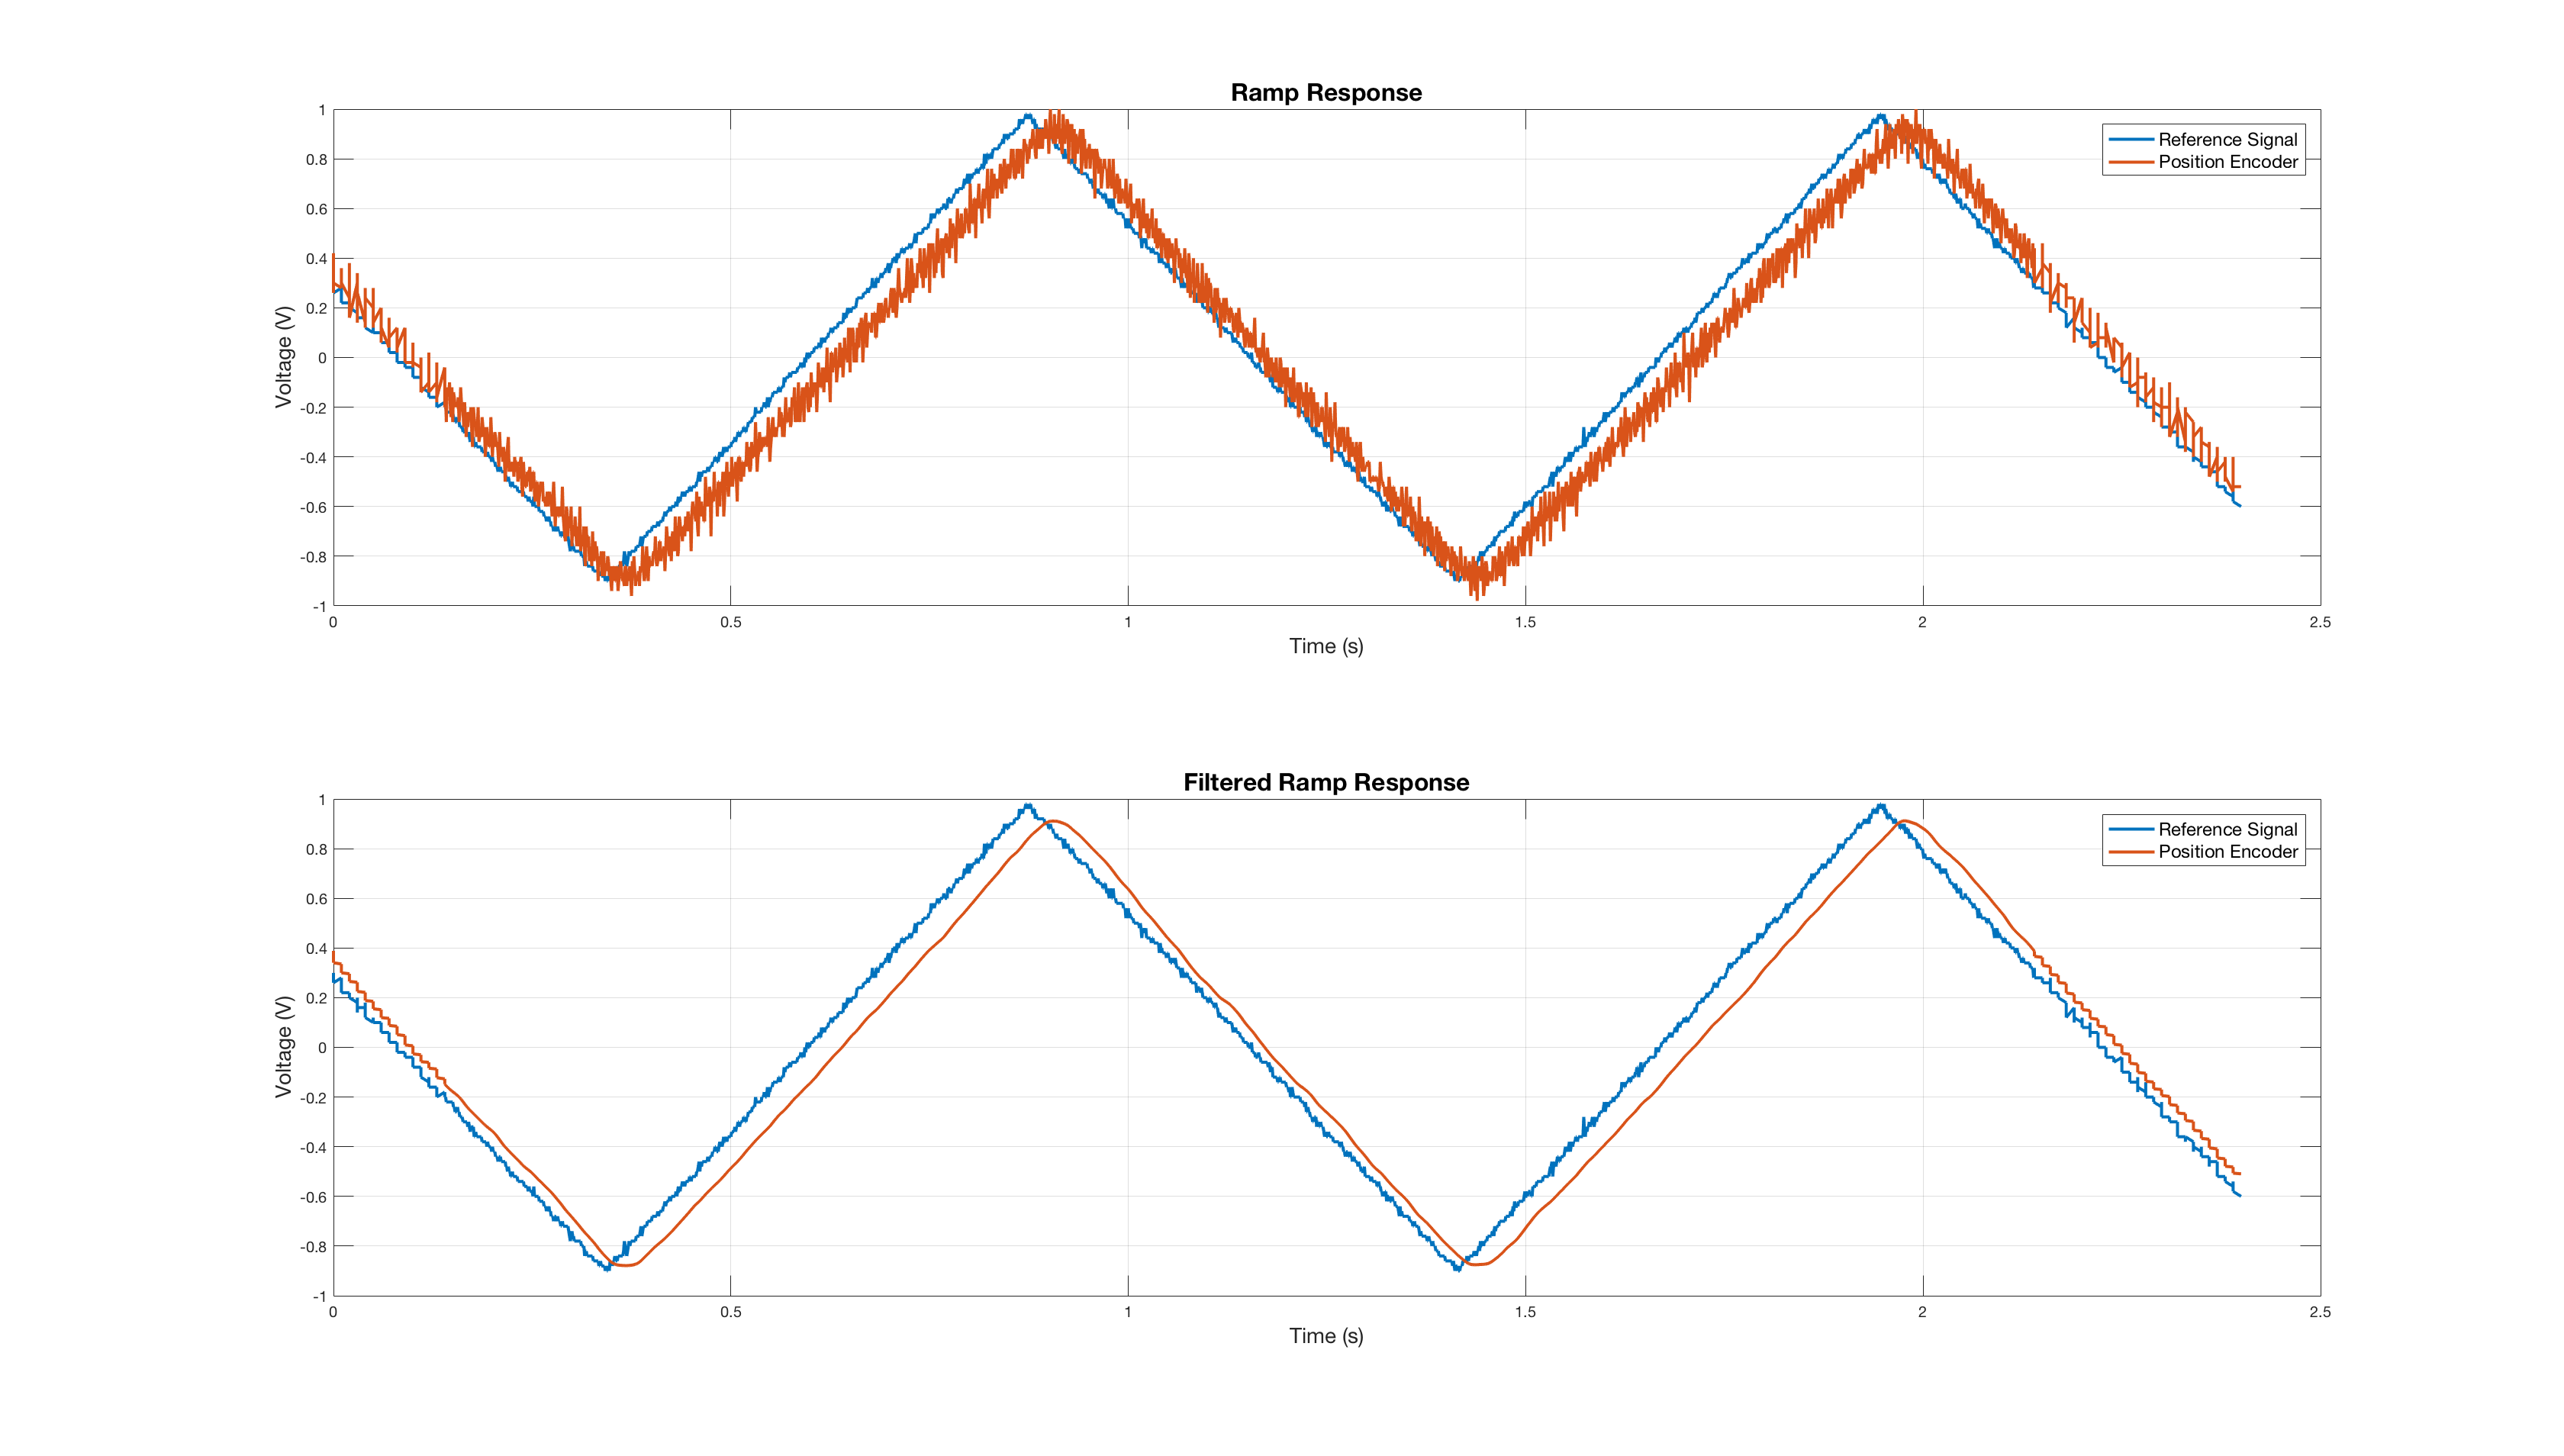
\includegraphics[width=1.1\textheight]{img/results/ramp.png}
    \label{fig::ramp_response}
    \caption{Resposta do sistema à entrada rampa unitária. O sinal de referência foi gerado por um gerador de sinais, de amplitude $1V$ pico a pico e $1Hz$. O sinal de posição do carro foi lido da saída PWM do sistema Arduino. Estão representados tanto o sinal original lido no osciloscópio, como um sinal filtrado para remover ruídos de alta frequência.}
\end{sidewaysfigure}
